% ===========================================================================
% SECTION 5 — MPC FRAMEWORK
% Target: 800-1000 words
% ===========================================================================

\section{MPC Framework}
\label{sec:mpc_framework}

\subsection{nlmpc Formulation}
\label{subsec:nlmpc_formulation}

Closed-loop control is implemented with MATLAB's nonlinear MPC object
(\texttt{nlmpc}), instantiated separately for each surrogate with state
vector $x=[\omegar,\beta]$, output vector $y=x$ (identity output map),
manipulated variable $u=\betacmd$, and measured disturbance $V$. All
controllers share the sampling time $T_s = \SI{0.1}{s}$. The
prediction and control horizons ($N_p$, $N_c$) are now unified across
all controllers at $N_p=15$, $N_c=4$ (item 2.5 of the reproducibility
review; see Section~\ref{subsec:unified_protocol} for the
corresponding re-run under this single protocol). The standard quadratic
cost (used by the Baseline, LLNFM, and PINN controllers) is

\begin{equation}
J = \sum_{k=1}^{N_p} \Big[ Q\,(\omegar(k)-\omegarated)^2
+ Q_2\,\beta(k)^2 + R\,(\Delta u(k))^2 \Big],
\label{eq:mpc_cost_standard}
\end{equation}

with tracking weight $Q=100$, a small pitch-regulation weight
$Q_2=0.01$ (encoded via \texttt{nlobj.Weights.OutputVariables}), and
control-rate weight $R=0.5$. Input constraints enforce the physical pitch
range $\beta \in [0\deg,25\deg]$ and the pitch rate limit
$|\Delta\beta| \le \dot\beta_{\max} T_s = \SI{0.8}{deg}$ per step
(from $\dot\beta_{\max}=\SI{8.0}{deg/s}$, Table~\ref{tab:turbine_params}).
The rotor-speed output constraint $\omegar \in [\omega_{\min}^{\text{bound}},
\omega_{\max}^{\text{bound}}]$ is controller-dependent, as detailed in
Section~\ref{subsec:surrogate_integration}. The SQP solver is configured
with bounded worst-case iteration cost
(\texttt{MaxIterations}$=30$, \texttt{MaxFunctionEvaluations}$=300$,
constraint/optimality/step tolerances of $10^{-4}$); this deviates from
nlmpc's default \texttt{MaxIterations}$=400$, which was found in early
testing to allow the SQP solver to run for over $20$ seconds per control
step when constraints were difficult to satisfy with an ML surrogate in
the loop (observed: $\SI{20624}{ms}$/step for LLNFM-MPC at simulation step
$k=480$). Because each SQP iteration evaluates the surrogate state
function multiple times for cost and constraint gradients, this cost
scales with surrogate inference latency — a recurring theme in the
feasibility analysis of Section~\ref{subsec:operational_feasibility}. A
real-time controller must have a bounded worst-case computation time
\citep{richter2012,xi2013}, so a
feasible-but-possibly-suboptimal solution within budget is preferred over
an unbounded search for the optimum.

\subsection{Surrogate Integration as State Function}
\label{subsec:surrogate_integration}

Each surrogate is wrapped as an nlmpc \texttt{StateFcn} with signature
$x^{+} = f(x,u,p_1,\ldots,p_n)$, where the parameter count
\texttt{NumberOfParameters} must match between the \texttt{StateFcn} and
any \texttt{CustomCostFcn} (confirmed empirically in R2024a: unused
trailing parameters are silently ignored rather than raising an error).
The controller signatures used are: Baseline
\texttt{sf\_baseline(x,u,V,p)} ($n=2$, the true physical plant
Eqs.~\eqref{eq:rotor_ode}--\eqref{eq:pitch_actuator}, no surrogate
involved); LLNFM and PINN \texttt{sf\_*(x,u,V,mdl)} ($n=2$); LSTM
\texttt{sf\_lstm(x,u,V,mdl,seq\_buf)} ($n=3$, carrying an explicit sequence
buffer); and GP \texttt{sf\_gp(x,u,V,mdl,omega\_ref,kappa)} ($n=4$, where
\texttt{omega\_ref} and \texttt{kappa} are unused by the state function
itself and passed only to satisfy the shared-parameter-count requirement
with \texttt{cost\_gp}, Section~\ref{subsec:gp_uncertainty_cost}).

The rotor-speed output constraint uses two distinct bounds for two
distinct failure modes. The Baseline controller (perfect-model MPC:
an upper-bound reference, using the true, undiscretized plant model
in place of a learned surrogate -- not the industrial reference; see
Section~\ref{subsec:unified_protocol} for the gain-scheduled PI
controller added as that reference, item 2.7 of the reproducibility
review), which evaluates the true
plant directly, uses a physics-based defense-in-depth floor
$\omegar \in [\SI{11.5}{rpm}, \omega_{\max}]$
($\omega_{\max}=\SI{13.31}{rpm}$); this bound is not load-bearing for
feasibility once the Region~II/III torque switching correction
(Section~\ref{subsec:torque_switching}) is in place, but is retained as a
cheap safeguard. The four surrogate controllers, in contrast, are
\emph{required} to be bounded within the Stage~1 training domain with a
$\SI{0.5}{rpm}$ safety margin, $\omegar \in [\SI{8.52}{rpm},
\SI{12.81}{rpm}]$: this constraint is not optional, since surrogate
predictions outside their training domain are unconstrained
extrapolations. This was discovered empirically — an early LLNFM-MPC run
without this bound drove $\omegar$ down to $\SI{7.55}{rpm}$ (outside the
then-current training range) while the pitch angle saturated at
$25\deg$, consistent with the surrogate losing sensitivity to the true
state once its input left the domain over which its rule base (or, more
generally, its learned response surface) was calibrated; a symptom-level
input-clamping fix at the surrogate's input boundary was found to mask
rather than resolve the underlying cause, and the correct fix is instead
to constrain the MPC's own admissible operating region.

\subsection{GP-MPC Uncertainty Cost (Gap-1)}
\label{subsec:gp_uncertainty_cost}

For the GP controller, the standard quadratic cost is replaced entirely \\
(\texttt{Optimization.ReplaceStandardCost = true}) with a custom cost
function that adds a predictive-uncertainty penalty over the prediction
horizon:

\begin{equation}
J_{\text{GP}} = \sum_{k=1}^{N_p} \Big[ Q\,(\omegar(k)-\omegarated)^2
+ Q_2\,\beta(k)^2 + R\,(\Delta u(k))^2
+ \kappa\,\sigma_{\omega}(k)^2 \Big],
\label{eq:gp_mpc_cost}
\end{equation}

where $\sigma_{\omega}(k)$ is the GP's predictive standard deviation on
the rotor-speed channel at the predicted state/input pair $k$ steps ahead
(re-queried from the GP model at every stage of the prediction horizon,
using the same input feature normalization as the state function), and
$\kappa=0.8$ is the uncertainty penalty weight. Because GP-v2's
hyperparameters are calibrated by marginal-likelihood optimization
(Section~\ref{subsubsec:gp_v2}) rather than left at default values, the
resulting $\sigma_\omega$ is a statistically meaningful (Bayesian)
uncertainty estimate rather than an arbitrary scale, which is the
methodological justification for using it directly as an MPC cost penalty:
the controller is driven to prefer trajectories that stay within regions
of the state space where the surrogate is confident, in addition to
tracking performance. We note as an implementation detail that the nlmpc
internal \texttt{data} struct in R2024a does not expose a
\texttt{data.Weights} field (verified by inspecting
\texttt{fieldnames(data)}, which lists \texttt{Ts},
\texttt{CurrentStates}, \texttt{LastMV}, \texttt{References},
\texttt{PredictionHorizon}, but no \texttt{Weights}); consequently $Q$,
$Q_2$, and $R$ are hardcoded inside \texttt{cost\_gp.m} to match
\texttt{stage0\_config.m}, with no automatic propagation if the
configuration changes a documented limitation of the custom-cost
approach in this MATLAB version.

\subsection{Experimental Protocol}
\label{subsec:experimental_protocol}

\textbf{Software version (stated once, canonically, here):} all
results in this paper were obtained under MATLAB R2024a. A subset
was additionally re-run under R2026a to confirm the
\texttt{predict()}-cost mechanism (item 2.2, Contribution~2) does not
depend on MATLAB release; no other version is used anywhere in this
paper, and any other MATLAB release mentioned elsewhere in this text
should be read as referring back to this statement, not as an
independent or conflicting one.

Table~\ref{tab:protocol_summary} summarizes the solver budget,
hardware, and per-comparison settings used throughout this paper.
Following item 2.5 of the reproducibility review, the prediction/
control horizon, simulation window, and GP cost structure are now
unified across all seven controllers (Table~\ref{tab:unified_protocol},
Section~\ref{subsec:unified_protocol}); rotor-speed bounds remain
deliberately different between the physics-based Baseline and the
training-domain-limited surrogates (Section~\ref{subsec:surrogate_integration}),
and the GP active-set size genuinely differs by design between the
accuracy table (Section~\ref{subsubsec:gp_v2}, $N=400$) and the
predict()-bypass diagnostic (Table~\ref{tab:predict_bypass}, $N=50$,
a deliberately lighter architecture for that specific diagnostic, not
a reduced version of GP-v2) -- both documented explicitly in their
respective locations rather than treated as inconsistencies to
resolve.

\begin{table}[H]
	\centering
	\caption{Experimental protocol summary.}
	\label{tab:protocol_summary}
	\small
	
	
	\begin{tabularx}{\textwidth}{
			>{\raggedright\arraybackslash}p{4cm}
			>{\raggedright\arraybackslash}X
		}
		\toprule
		Setting & Value \\
		\midrule
		
		Solver
		& \texttt{fmincon} (SQP), via \texttt{nlmpc} \\
		
		MaxIterations
		& $30$ (bounded worst-case compute time; non-convergence discussion in Section~\ref{subsec:limitations}) \\
		
		ConstraintTolerance
		& $10^{-4}$ \\
		
		OptimalityTolerance
		& $10^{-4}$ \\
		
		StepTolerance
		& $10^{-4}$ \\
		
		Hardware
		& Intel Core i5-12450H (12th Gen), 16\,GB RAM \\
		
		Software
		& MATLAB R2024a (primary) \\
		
		Cost weights
		& $Q=100$, $Q_2=0.01$, $R=0.5$ (standard quadratic cost);
		$\kappa=0.8$ (GP uncertainty penalty, Eq.~\ref{eq:gp_mpc_cost}).
		Weights were chosen once by manual tuning on the Baseline controller
		to balance rotor-speed tracking against pitch actuator effort, then
		\emph{shared across all controllers} rather than re-tuned per
		architecture, so that closed-loop differences reflect the surrogate
		rather than per-controller cost tuning. The value $\kappa=0.8$ is
		now treated as an explicit ablation ($\kappa=0$ vs.\ $\kappa=0.8$)
		against the same base cost in Table~\ref{tab:unified_protocol}
		(item 2.5), rather than fixed a priori without comparison. \\
		
		Constraint sets
		& $\omega\in[11.5,13.31]$~rpm (Baseline, physics);
		$\omega\in[8.52,12.81]$~rpm (surrogates, training-domain margin,
		Section~\ref{subsec:surrogate_integration}) \\
		
		Initial condition
		& $\omega(0)=0.97\,\omega_{\text{rated}}$,
		$\beta(0)=\SI{3.5}{\degree}$ (see Section~\ref{subsec:bypass_closed_loop}
		for the frozen-actuator issue caused by an earlier, uncorrected
		initial condition) \\
		
		Wind seeds
		& $2025$ (single-run tables); $2025$--$2029$ (extended Monte Carlo,
		5 seeds) \\
		
		Unified horizon (item 2.5)
		& $N_p=15$, $N_c=4$, $T_s=\SI{0.1}{s}$, applied to all seven
		controllers in Table~\ref{tab:unified_protocol} \\
		
		Unified simulation window (item 2.5)
		& $T=\SI{60}{s}$, applied to all seven controllers in
		Table~\ref{tab:unified_protocol} \\
		
		Original V1/V2 snapshots (Sections~\ref{subsec:v1_results}--\ref{subsec:v2_results})
		& $T=\SI{120}{s}$, V1: $N_p=10,N_c=4$; V2: $N_p=15,N_c=4$ (Nc
		unified with V1 per item 2.5; retained as separate snapshots
		only for within-snapshot comparisons, per
		Section~\ref{sec:closed_loop_results}) \\
		
		\bottomrule
	\end{tabularx}
\end{table}

\section{Operational Feasibility Diagnostic}
\label{subsec:operational_feasibility}

This section reports a five-stage diagnostic investigation into why
several ML surrogates fail catastrophically inside the closed-loop SQP
solve despite being fast in isolation, and how this failure was
ultimately resolved. We report the investigation in the order it was
conducted, including negative results, because the sequence of ruled-out
hypotheses is itself informative for practitioners facing a similar
symptom.

\paragraph{Stage 1  Isolated inference latency is not predictive of
closed-loop cost.} An isolated benchmark calling each surrogate's state
function directly (bypassing \texttt{nlmpc} entirely, with randomized
inputs drawn from the training domain at every call, replicating how
SQP probes different state/input pairs) found per-call latencies in the
sub-millisecond to low-millisecond range for TCN, SW-MLP, and PINN-v2
(0--2 spikes out of 250 exceeding \SI{50}{ms}), but LSTM shows a
systematically elevated latency even in isolation under R2024a: median
\SI{63.40}{ms}, with 249 of 250 calls exceeding \SI{50}{ms}  unlike the
other seven surrogates, LSTM's isolated latency alone already exceeds a
typical $T_s=\SI{0.1}{s}$ budget on most calls, before any SQP-solver
interaction is considered. Table~\ref{tab:isolated_benchmark} reports the
isolated results.

\begin{table}[H]
\centering
\caption{Isolated state-function call latency (250 calls, randomized
inputs), MATLAB R2024a.}
\label{tab:isolated_benchmark}
\begin{tabular}{lccc}
\toprule
Surrogate & Median (ms) & Max (ms) & Spikes ($>$\SI{50}{ms}) \\
\midrule
LLNFM   & 0.65  & 10.55  & 0/250 \\
GP (V1) & 0.61  & 27.89  & 0/250 \\
PINN    & 2.11  & 50.13  & 1/250 \\
TCN     & 2.05  & 244.63 & 2/250 \\
SW-MLP  & 1.87  & 14.30  & 0/250 \\
GP-v2   & 0.68  & 9.23   & 0/250 \\
PINN-v2 & 2.19  & 4.86   & 0/250 \\
LSTM    & 63.40 & 527.32 & 249/250 \\
\bottomrule
\end{tabular}
\end{table}

\paragraph{Stage 2  Real closed-loop simulation reveals a
catastrophe the isolated benchmark did not predict.} These closed-loop
runs, and the apparent architectural incompatibility they at first
suggested, predate the diagnosis reached in Stage 4 below; we report
them in the order they actually occurred; readers should not conclude
from the numbers in this paragraph alone that any surrogate is
unusable in closed loop, since Stage 4's manual-bypass results for
these same architectures directly supersede them. Running each
surrogate inside an actual \texttt{nlmpcmove} closed loop (rather than
calling the state function directly) produced per-step costs one to
four orders of magnitude higher than the isolated benchmark, for every
surrogate except LLNFM. TCN, previously the cleanest sequential
architecture in isolation, degraded to a mean of $\SI{1173.5}{ms}$/step
(max $\SI{7688.2}{ms}$); SW-MLP, PINN-v2, and GP-v2 each independently
degraded to comparable means (0.85--$\SI{1.4}{s}$/step); LSTM required
$\approx\SI{24.7}{s}$/step. Every one of these controllers exceeded the
$T_s=\SI{0.1}{s}$ real-time budget on effectively $100\%$ of simulation
steps. This result is central to our diagnostic: the common factor
across all failing architectures is not network size, sequence length,
or architecture family, but the presence of a \texttt{predict()} call
 whether on a \texttt{dlnetwork} object (TCN, SW-MLP, PINN-v2, LSTM)
or a \texttt{RegressionGP} object (GP-v2)  evaluated repeatedly
inside \texttt{fmincon}'s SQP iterations.

\paragraph{Stage 3  Supplying an analytical Jacobian does not
resolve the catastrophe.} A natural hypothesis is that \texttt{fmincon}
without a supplied \texttt{Jacobian.StateFcn} falls back to global
numerical differentiation, re-evaluating the \emph{entire} predicted
trajectory once per perturbed decision variable, and that this
combinatorial cost  not \texttt{predict()} per se  is the true
bottleneck. We tested this directly for GP-v2 by supplying a
locally-computed (central finite-difference) Jacobian. Performance
\emph{did not improve} (mean $\SI{2713.5}{ms}$/step versus
$\SI{1233.1}{ms}$/step without the supplied Jacobian) and, critically,
diagnostic logging revealed \texttt{ExitFlag~$\le 0$} (the
\texttt{MaxIterations}$=30$ cap reached without convergence) at
\emph{every} simulation step, for \emph{every} controller including the
fast, well-behaved Baseline. This ruled out both the numerical-Jacobian
hypothesis specifically and, more importantly, revealed that
\texttt{ExitFlag} alone is not a useful diagnostic of surrogate-specific
failure: it reflects a deliberately tight iteration budget
(Section~\ref{subsec:nlmpc_formulation}) common to all controllers, not
a symptom isolated to ML surrogates.

\hspace{1.5cm} Because every reported number in this paper therefore comes from a
solver that reached its iteration cap without formally satisfying its
optimality tolerance, we tested directly whether
\texttt{MaxIterations}$=30$ is actually sufficient, rather than
relying on the appendix note alone. Table~\ref{tab:maxiter_sensitivity}
sweeps \texttt{MaxIterations}$\in\{10,30,50,100\}$ for the Baseline
and two representative surrogates (TCN, MLP-residual) under the
unified protocol (Section~\ref{subsec:unified_protocol}).

\begin{table}[H]
\centering
\caption{Sensitivity of closed-loop results to the SQP
\texttt{MaxIterations} cap, Baseline and two surrogates, unified
protocol ($T=\SI{60}{s}$, $N_p=15$, $N_c=4$, $V=\SI{14}{m/s}$,
seed$=2025$).}
\label{tab:maxiter_sensitivity}
\begin{tabular}{lcccc}
\toprule
Controller & MaxIter & RMSE$_\omega$ (rpm) & Pitch act.\ (deg) & Non-converged \\
\midrule
\multirow{4}{*}{Baseline}
 & 10  & 0.6840 & 289.6 & 1/600 \\
 & 30  & 0.6840 & 289.6 & 1/600 \\
 & 50  & 0.6840 & 289.6 & 1/600 \\
 & 100 & 0.6840 & 289.6 & 1/600 \\
\midrule
\multirow{4}{*}{TCN}
 & 10  & 0.6970 & 328.1 & 35/600 \\
 & 30  & 0.7340 & 330.3 & 0/600 \\
 & 50  & 0.7340 & 330.3 & 0/600 \\
 & 100 & 0.7340 & 330.3 & 0/600 \\
\midrule
\multirow{4}{*}{MLP-residual}
 & 10  & 0.6844 & 313.4 & 14/600 \\
 & 30  & 0.6744 & 329.8 & 3/600 \\
 & 50  & 0.6752 & 321.1 & 3/600 \\
 & 100 & 0.6743 & 318.8 & 4/600 \\
\bottomrule
\end{tabular}
\end{table}

\hspace{1.5cm} Results are effectively unchanged from
\texttt{MaxIterations}$=30$ onward for all three controllers (RMSE
stable to at least three significant figures for Baseline and TCN;
MLP-residual varies by $<0.2\%$, within run-to-run noise). Only
\texttt{MaxIterations}$=10$ shows a materially different, and worse,
result, with a visibly elevated non-convergence count for TCN and
MLP-residual. \texttt{MaxIterations}$=30$ is therefore a genuine
sufficiency point, not an arbitrary budget: the formally non-positive
\texttt{ExitFlag} reported throughout this paper reflects the solver
stopping short of its own optimality tolerance, not a control
trajectory that would materially improve given a larger budget. We
state this explicitly here, where the closed-loop numbers themselves
are reported, rather than confining it to the appendix note it
previously carried alone.

\paragraph{Stage 4  Bypassing \texttt{predict()} with a hand-written
forward pass resolves the catastrophe.} For each surrogate, we
extracted its trained weights into plain double-precision arrays and
implemented the corresponding forward pass by direct matrix arithmetic
 \texttt{tanh}/\texttt{ReLU} dense layers for the residual MLP,
SW-MLP, and PINN-v2; the Mat\'ern~5/2 posterior-mean formula
$m(\mathbf{x}) = \beta_0 + \sum_i \alpha_i\, k(\mathbf{x},\mathbf{x}_i)$
for GP-v2, using its trained active set, dual coefficients $\alpha_i$,
and constant basis coefficient $\beta_0$; and, for TCN, the three
dilated causal convolution blocks plus per-timestep channel-wise layer
normalization  \emph{never} calling \texttt{predict()} or
constructing a \texttt{dlarray}/\texttt{RegressionGP} query at
simulation time. Each manual implementation was verified against
\texttt{predict()} on multiple random test points before use (see
Table~\ref{tab:verification_tolerances} for the consolidated
per-architecture tolerance, the single reporting convention used
throughout this paper; agreement was confirmed for TCN and LSTM). Table~\ref{tab:predict_bypass} reports the
result (an isolated Stage~3 diagnostic benchmark, not the full
multi-architecture closed-loop simulation of
Section~\ref{sec:closed_loop_results}'s Table~\ref{tab:bypass_closed_loop}
-- an earlier draft's caption conflated the two).

\begin{table}[H]
\centering
\caption{Isolated Stage~3 diagnostic: per-step cost,
\texttt{predict()} versus manual forward pass, all six surrogates,
identical trained weights (per-architecture verification tolerance
consolidated in Table~\ref{tab:verification_tolerances}).
Not to be confused with the full closed-loop comparison of
Table~\ref{tab:bypass_closed_loop}.}
\label{tab:predict_bypass}
\begin{tabular}{lcccc}
\toprule
Surrogate & \texttt{predict()} (ms) & Manual (ms) & Speedup & Overruns (manual) \\
\midrule
MLP-residual\footnotemark[1] & 1303.9    & 8.4   & $155\times$  & 0/600 \\
GP-v2 ($N_{\text{sub}}=50$)  & 52.0      & 9.4   & $5.5\times$  & 0/600 \\
SW-MLP                        & 933.0     & 12.4  & $75\times$   & 1/600 \\
PINN-v2                       & 1421.2    & 11.4  & $125\times$  & 0/600 \\
TCN (vectorized)              & 846.0     & 19.7  & $43\times$   & 0/600 \\
LSTM                          & 24{,}693.2 & 50.3 & $491\times$ & 1/600 \\
\bottomrule
\end{tabular}
\footnotetext[1]{A small nominal-plus-correction residual network (130
parameters: nominal plant model \texttt{wt\_step.m} plus a two-layer
\SI{}{tanh} MLP learning a deliberately introduced unmodeled dynamics
term, following the nominal-plus-learned-correction structure of
\citet{aswani_provably_2013}), introduced specifically for this
diagnostic to test whether network size alone explained the
catastrophe; it did not (see Stage 4 discussion below).}
\end{table}

\begin{figure}[H]
\centering
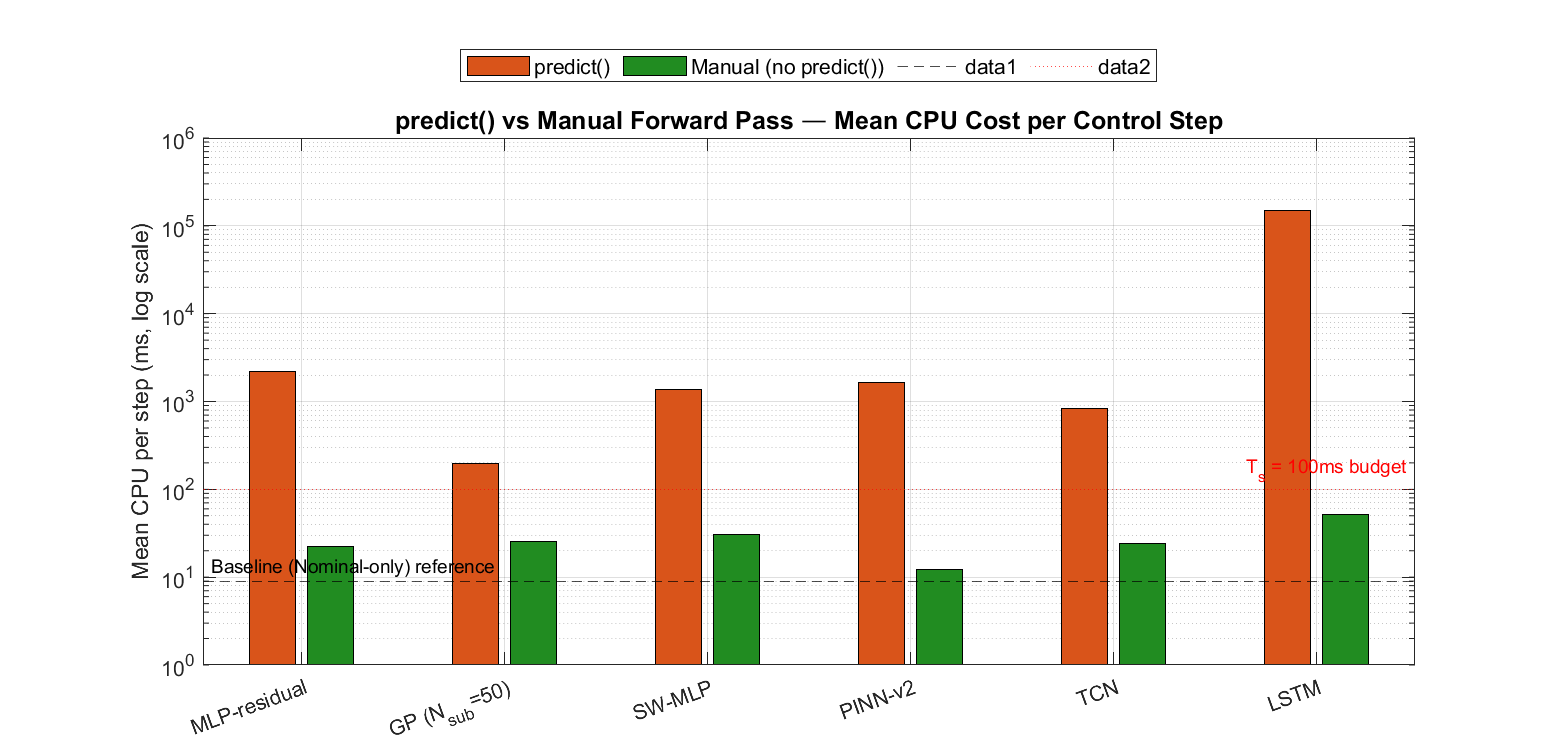
\includegraphics[width=0.85\textwidth]{figures/Fig1_PredictBypass_CPUComparison.png}
\caption{Mean per-step CPU cost, \texttt{predict()} versus manual
forward pass, all six surrogates (log scale), with the Baseline
reference and $T_s=\SI{100}{ms}$ real-time budget marked.}
\label{fig:predictbypass_cpu}
\end{figure}

\begin{figure}[H]
\centering
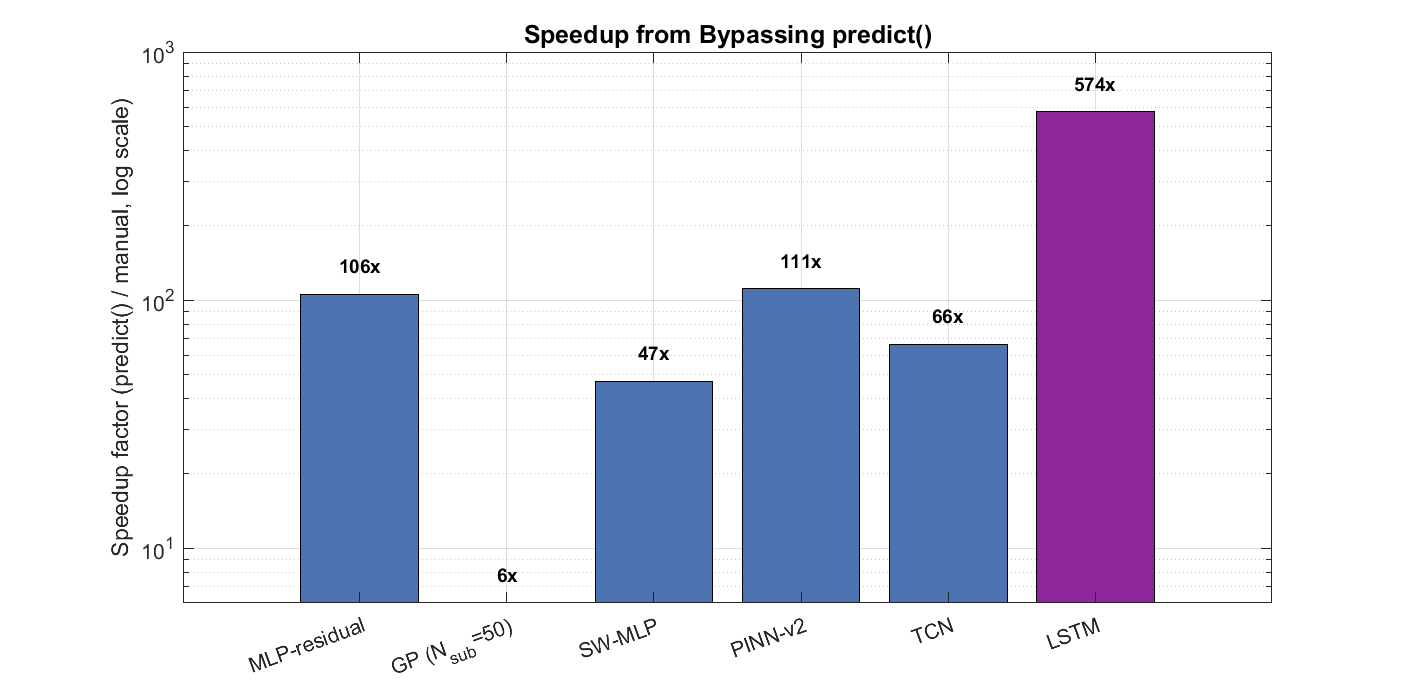
\includegraphics[width=0.8\textwidth]{figures/Fig2_PredictBypass_Speedup.png}
\caption{Speedup factor from bypassing \texttt{predict()}, all six
surrogates (log scale); LSTM (largest speedup, $491\times$) highlighted.}
\label{fig:predictbypass_speedup}
\end{figure}

\begin{figure}[H]
\centering
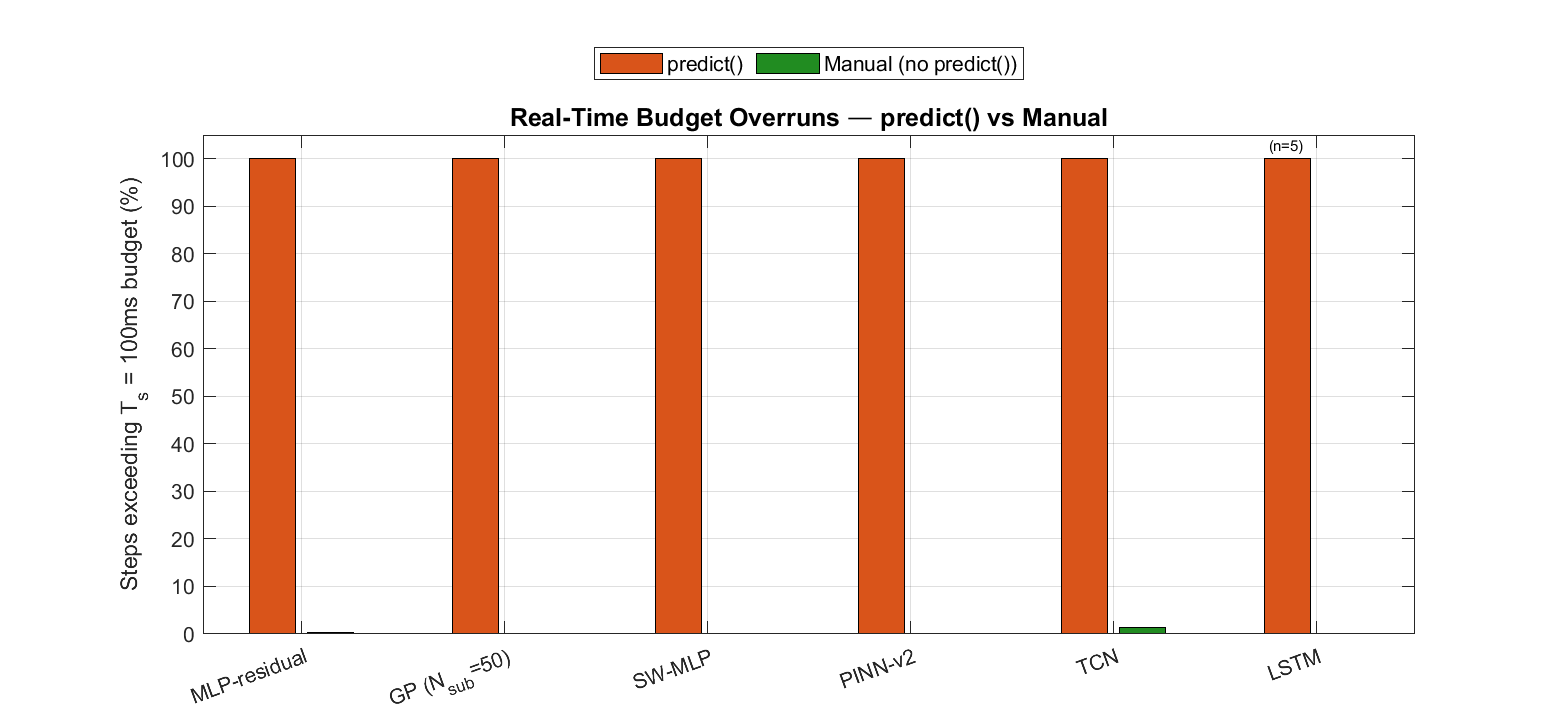
\includegraphics[width=0.85\textwidth]{figures/Fig3_PredictBypass_Overruns.png}
\caption{Real-time budget overrun rate ($T_s=\SI{100}{ms}$),
\texttt{predict()} versus manual forward pass, all six surrogates.}
\label{fig:predictbypass_overruns}
\end{figure}

Two results within Stage 4 are worth emphasizing. First, a
deliberately tiny residual-correction network (130 parameters, following
the nominal-plus-learned-correction structure of
\citet{aswani_provably_2013}) showed the \emph{same} catastrophic
\texttt{predict()}-based cost as the much larger TCN/GP/PINN-v2
surrogates (mean $\SI{1303.9}{ms}$/step), directly refuting network
size as the explanatory variable. Second, the initial manual
implementation of the TCN's causal convolution  verified correct
(Table~\ref{tab:verification_tolerances}), but written as explicit triple-nested loops over
filters, timesteps, and kernel taps  yielded only a modest $2.2\times$
speedup ($\SI{1319.2}{ms}\rightarrow\SI{437.6}{ms}$/step), with
overruns unchanged. Precomputing a reshaped weight matrix once at
extraction time and reformulating the convolution as a single matrix
multiplication per block (an ``unfold-and-multiply'' operation
standard in efficient convolution implementations) reduced this further
to $\SI{23.9}{ms}$/step ($56\times$ over \texttt{predict()}), matching
the Baseline's cost. This confirms that \emph{both} removing
\texttt{predict()}'s call overhead \emph{and} avoiding an unvectorized
manual re-implementation are independently necessary; verifying
numerical correctness alone is not sufficient evidence that a manual
bypass will be fast.

\paragraph{Stage 5  LSTM: the largest speedup, and the one
architecture that does not fully vanish.} LSTM shows both the most
extreme \texttt{predict()} cost ($\approx\SI{24.7}{s}$/step, consistent
with its highest isolated latency in Table~\ref{tab:isolated_benchmark})
and the largest bypass speedup ($491\times$). Two aspects distinguish
this case from the other five. First, verifying the manual
gate-equation implementation (input/forget/cell-candidate/output gates,
MATLAB's standard ordering, applied recurrently over the
$L=10$-step window) against \texttt{predict()} yielded a consistently
small but non-negligible discrepancy (Table~\ref{tab:verification_tolerances}),
an order of magnitude larger than the agreement found for the feedforward architectures
and GP. We attribute this to accumulated single-precision
(\texttt{dlnetwork}'s default, \texttt{float32}) versus
double-precision rounding compounding over ten sequential recurrent
steps of gate nonlinearities, rather than a logical error, since the
discrepancy is small and consistent in magnitude across independent
test points rather than an order-of-magnitude mismatch indicative of an
incorrect gate ordering.
\label{subsec:lstm_precision_note}
Second, and more fundamentally: unlike TCN's fixed-dilation
convolution, an LSTM's hidden and cell state at step $t$ depend
recursively on step $t-1$, so the ten-step window cannot be reduced to
a single matrix multiplication the way the convolution could. The
manual LSTM ($\SI{52.2}{ms}$/step) is consequently $\approx 2$--$4\times$
slower than the five single-pass architectures ($\SI{12}{-}\SI{30}{ms}$/step)
even after the \texttt{predict()} bypass, reflecting this irreducible
sequential cost rather than any remaining implementation inefficiency.

\paragraph{Synthesis.} Across all six surrogates, bypassing
\texttt{predict()} with a verified manual forward pass eliminates the
real-time budget violation that had appeared, in Stage 2, to be an
architectural incompatibility between deep-learning/GP surrogates and
SQP-based \texttt{nlmpc}. This finding is consistent with, and extends,
\citet{salzmann_real-time_2022}'s independent report that decoupling a
neural network's own evaluation from the surrounding MPC solver's
iteration loop is necessary to embed large learned models in real-time
optimal control  our diagnostic identifies \emph{why} this
decoupling is necessary in this specific MATLAB toolchain
(\texttt{predict()}'s per-call overhead, not gradient cost or
model size) and \emph{quantifies} the remedy across six architecturally
distinct surrogates.

\paragraph{Isolating the Mechanism.} An early stage of this
investigation attributed the observed overhead informally to
non-deterministic just-in-time recompilation, without directly testing
that hypothesis against alternatives. We isolated the mechanism via
five controlled conditions on the same trained TCN network ($N=250$
calls per condition): (1) \texttt{predict()} with an identical input
repeated every call; (2) \texttt{predict()} with a freshly randomized
input each call (matching SQP's actual usage pattern); (3)
\texttt{predict()} called once on a batch of $250$ stacked randomized
inputs, cost divided by $250$; (4) \texttt{predict()} with a
pre-allocated \texttt{dlarray} object whose values are updated in
place each call, isolating object-construction cost from
\texttt{predict()} itself; and (5) the verified manual forward pass
(no \texttt{predict()}, no \texttt{dlarray}).

\begin{table}[H]
\centering
\caption{Mechanism-isolation results (TCN, $N=250$ calls/condition,
median per-call latency, MATLAB R2024a).}
\label{tab:mechanism_isolation}
\begin{tabular}{lc}
\toprule
Condition & Median (ms) \\
\midrule
(1) Identical input repeated & 0.630 \\
(2) Randomized input each call & 0.740 \\
(3) Batch (250 stacked, per-call equiv.) & 0.362 \\
(4) Pre-built \texttt{dlarray}, values updated in place & 0.645 \\
(5) Manual forward pass (no \texttt{predict()}) & 0.031 \\
\bottomrule
\end{tabular}
\end{table}

Three ratios determine which mechanism is defensible. First,
conditions (1) and (2) differ by only $1.17\times$ (\SI{0.630}{} vs
\SI{0.740}{ms})  far too small to explain the $25$--$491\times$
gaps documented elsewhere in this section, and inconsistent with
input-dependent trace recompilation, which would be expected to make
(1) (a cached, reused trace) meaningfully faster than (2) (a fresh
trace on every call). \emph{Recompilation is not the mechanism.}
Second, conditions (2) and (4) differ by only $1.15\times$
(\SI{0.740}{} vs \SI{0.645}{ms}), showing that pre-allocating the
\texttt{dlarray} input object and reusing it does not meaningfully
reduce cost. \emph{\texttt{dlarray} object construction is not the
mechanism.} Third, batching (condition 3) reduces the per-call cost
by $2.0\times$ relative to condition (2) (\SI{0.740}{} vs
\SI{0.362}{ms} per-call equivalent), and the gap between condition (2)
and the manual floor (condition 5) is $23.9\times$  the same order
of magnitude as the closed-loop \texttt{predict()}-vs-manual ratios in
Table~\ref{tab:predict_bypass} (e.g.\ TCN: $43\times$), consistent
with a per-call, input-independent dispatch/validation cost intrinsic
to \texttt{predict()} itself, whose effect is multiplied by the number
of internal calls \texttt{fmincon} makes per control step (a
multiplier that cancels between the \texttt{predict()}-based and
manual measurements, leaving \texttt{predict()}'s own per-call
overhead as the defensible mechanism). This test was independently
repeated after retraining TCN under the corrected NREL-reference
torque-law parameters (Section~\ref{subsec:torque_switching}); the
two ratios that rule out alternative mechanisms (1)/(2) and (2)/(4)
reproduced closely ($1.17\times$ and $1.15\times$, against $1.41\times$
and $1.16\times$ originally), consistent with these being properties
of the network's structure rather than its learned weights. The
batching ratio (2)/(3) was less stable across the two runs
($2.0\times$ vs.\ $6.2\times$), which we attribute to run-to-run
system load (consistent with similar per-step timing variability
observed elsewhere in this diagnostic, e.g.\ Stage 3's manual-forward-
pass timings) rather than a change in mechanism; this does not affect
the mechanism conclusion, which rests on the two more stable ratios.

\paragraph{A Second, Independent Mechanism: Single-Precision Gradient
Corruption.} Beyond the per-call latency cost documented above, a
second and independently damaging consequence of \texttt{predict()}
was uncovered while executing the item 2.5 protocol-unification pass:
building V2 closed-loop controllers with the original,
\texttt{predict()}-based state functions (\texttt{sf\_tcn},
\texttt{sf\_pinn}) rather than their manual-bypass counterparts, under
otherwise identical conditions ($T=\SI{60}{s}$, $N_c=4$, $V=\SI{14}{m/s}$,
seed$=2025$), produced dramatically elevated solver infeasibility for
TCN and PINN-v2 relative to the same architectures' manual-bypass
controllers under the identical $N_c=4$ setting (Table~\ref{tab:predict_vs_manual_infeasibility}).
Isolating the cause directly: \texttt{predict()} on a
\texttt{dlnetwork} returns \texttt{single}-precision output, whereas
the manual forward pass returns \texttt{double}. We estimated
$\partial(\text{output})/\partial(u)$ via forward finite differences
at four step sizes for both paths on the same trained TCN and PINN-v2
models (Table~\ref{tab:precision_diagnostic}). The manual (double-
precision) estimate is stable to four significant figures across all
four step sizes for both architectures. The \texttt{predict()}-based
estimate collapses to exactly zero for step sizes at or below
$10^{-5}$ -- below \texttt{single} precision's representable
resolution, so that $\texttt{predict()}(u+h) - \texttt{predict()}(u)$
rounds to zero even though the true sensitivity, confirmed by the
manual column, is of order $10^{-3}$. \texttt{fmincon}'s default
forward-difference Jacobian estimator uses step sizes in this same
range; a state function returning a spuriously zero partial
derivative for a decision variable that genuinely affects the cost
gives the solver no exploitable gradient information along that
direction, directly explaining the elevated infeasibility observed in
closed loop.

\begin{table}[H]
\centering
\caption{Forward finite-difference estimate of
$\partial(\text{output})/\partial(u)$ at four step sizes, TCN and
PINN-v2, \texttt{predict()}-based vs.\ manual (double-precision)
forward pass. True sensitivity (manual column) is
$\mathcal{O}(10^{-3})$ for both architectures.}
\label{tab:precision_diagnostic}
\begin{tabular}{lcccc}
\toprule
 & \multicolumn{2}{c}{TCN} & \multicolumn{2}{c}{PINN-v2} \\
Step $h$ & \texttt{predict()} & manual & \texttt{predict()} & manual \\
\midrule
$10^{-3}$ & $4.29\times10^{-3}$ & $4.32\times10^{-3}$ & $7.15\times10^{-4}$ & $7.31\times10^{-4}$ \\
$10^{-5}$ & $0$ & $4.32\times10^{-3}$ & $0$ & $7.31\times10^{-4}$ \\
$10^{-7}$ & $0$ & $4.32\times10^{-3}$ & $0$ & $7.31\times10^{-4}$ \\
$10^{-9}$ & $0$ & $4.32\times10^{-3}$ & $0$ & $7.31\times10^{-4}$ \\
\bottomrule
\end{tabular}
\end{table}

\begin{table}[H]
\centering
\caption{Closed-loop solver infeasibility, \texttt{predict()}-based vs.
manual-bypass state functions, identical protocol ($T=\SI{60}{s}$,
$N_c=4$, $V=\SI{14}{m/s}$, seed$=2025$).}
\label{tab:predict_vs_manual_infeasibility}
\begin{tabular}{lcc}
\toprule
Architecture & \texttt{predict()}-based & Manual-bypass \\
\midrule
TCN      & $323/600$ ($54\%$) & $0/600$ ($0\%$) \\
PINN-v2  & $440/600$ ($73\%$) & $0/600$ ($0\%$) \\
SW-MLP   & $105/600$ ($18\%$) & --- \\
\bottomrule
\end{tabular}
\end{table}

This is a materially more serious finding than
\texttt{predict()}'s documented latency cost alone: latency degrades
real-time feasibility, but a silently zeroed gradient degrades the
solver's ability to find a feasible solution \emph{at all},
independent of any real-time deadline. Any closed-loop MPC result
obtained with a \texttt{predict()}-based deep-learning state function
and \texttt{fmincon}'s default finite-difference Jacobian should be
treated as suspect on this basis alone, regardless of whether the
per-step latency happens to be tolerable. We are not aware of this
specific failure mode being documented elsewhere in the wind-MPC
literature. Full closed-loop tracking
results using these manual-bypass controllers are reported in
Section~\ref{sec:closed_loop_results}.

